% Created 2021-04-10 Sat 23:41
% Intended LaTeX compiler: pdflatex
\documentclass[presentation,bigger,aspectratio=169]{beamer}
\usepackage[utf8]{inputenc}
\usepackage[T1]{fontenc}
\usepackage{graphicx}
\usepackage{grffile}
\usepackage{longtable}
\usepackage{wrapfig}
\usepackage{rotating}
\usepackage[normalem]{ulem}
\usepackage{amsmath}
\usepackage{textcomp}
\usepackage{amssymb}
\usepackage{capt-of}
\usepackage{hyperref}
\usepackage{xcolor}
\usepackage[]{minted}
\usepackage{tcolorbox}
\usepackage{etoolbox}\tcbuselibrary{magazine}
\BeforeBeginEnvironment{minted}{\begin{tcolorbox}[title=Input,colback=blue!5,colframe=blue!25!black,size=fbox, enforce breakable, break at=6cm]}%
\AfterEndEnvironment{minted}{\end{tcolorbox}}%
\BeforeBeginEnvironment{verbatim}{\begin{tcolorbox}[colback=white,size=fbox,enhanced jigsaw, enforce breakable,break at=6cm]}%
\AfterEndEnvironment{verbatim}{\end{tcolorbox}}%
\usepackage{inconsolata}
\usepackage[ngerman, germanb]{babel}
\usepackage [autostyle, english = american]{csquotes} \MakeOuterQuote{"}
\usepackage[utf8]{inputenc}\usepackage{tabulary,booktabs}\AtBeginEnvironment{tabulary}{\scriptsize}
\usepackage[fixlanguage]{babelbib}\selectbiblanguage{german}
\usepackage{csquotes,xpatch}\usepackage[natbib=true,style=apa,url=true,doi=true,annotation=false,eprint=false,backend=biber]{biblatex}\urlstyle{sf}
\DeclareLanguageMapping{austrian}{austrian-apa}
\DeclareSourcemap{\maps[datatype=bibtex]{\map{\step[fieldset=annotation,null]}}}\renewcommand*{\bibfont}{\scriptsize}
\addbibresource{~/Dropbox/org/ref/ref.bib}
%Global Background must be put in preamble
\usebackgroundtemplate%
{%
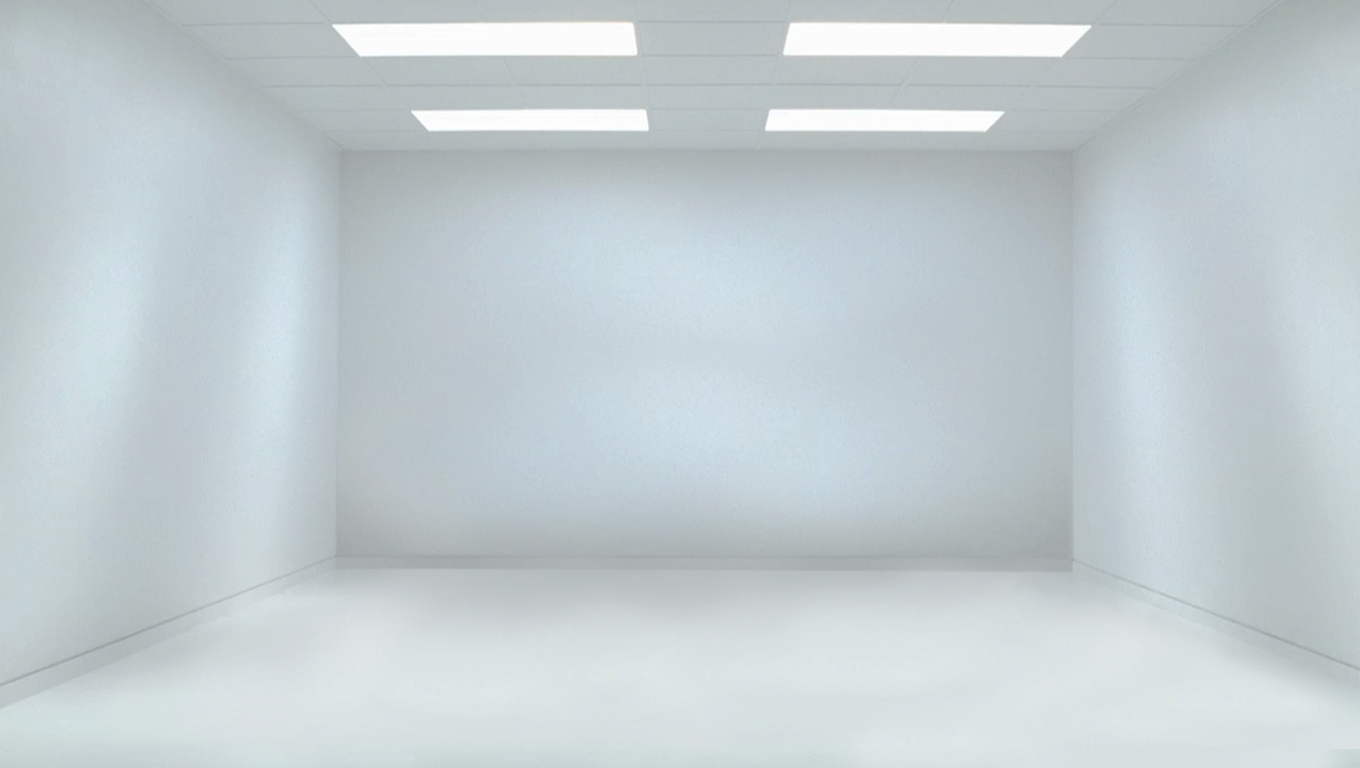
\includegraphics[width=1.175\paperwidth,height=\paperheight]{./img/m1_praes_empty_10.jpg}%
}
\usetheme{default}
\author{user\thanks{user@mink}}
\date{15.4.2021}
\title{M1}
\subtitle{Problemanalyse}
\usetheme{Hannover}\usepackage{graphicx}\usepackage[overlay]{textpos}
\setbeamertemplate{bibliography item}{}
\setbeamertemplate{navigation symbols}{}
\definecolor{UBCblue}{HTML}{153a7a}\usecolortheme[named=UBCblue]{structure}
\usefonttheme{professionalfonts}
\setbeamerfont{note page}{family*=pplx,size=\footnotesize}
\definecolor{bgminted}{HTML}{eee9e9}
\definecolor{bluegray}{rgb}{0.54, 0.6, 0.8}
\definecolor{urlcolor}{HTML}{3399ff}
\definecolor{linkcolor}{HTML}{3399ff}
\definecolor{colorlinkscolor}{HTML}{3399ff}
\hypersetup{colorlinks=colorlinkscolor,linkcolor=linkcolor,urlcolor=urlcolor}
\setbeamertemplate{itemize items}[default]
\setbeamertemplate{enumerate items}[default]
\setbeamertemplate{items}[default]
\setbeamerfont*{title in sidebar}{shape=\scshape,size=\scriptsize}
\setbeamerfont*{author in sidebar}{family=\sfseries,size=\scriptsize}
\setbeamerfont*{section in sidebar}{family=\sfseries,size=\scriptsize}
\usetheme{Hannover}
\def\swidth{3.6cm}
\setbeamersize{sidebar width left=\swidth}
\setbeamertemplate{sidebar left}
{
{\usebeamerfont{title in sidebar}%
\vskip1.5em%
\usebeamercolor[fg]{title in sidebar}%
\insertshorttitle[width=\swidth,center,respectlinebreaks]\par%
\vskip1.25em%
}%
{%
\usebeamercolor[fg]{author in sidebar}%
\usebeamerfont{author in sidebar}%
\insertshortauthor[width=\swidth,center,respectlinebreaks]\par%
\vskip1.25em%
}%
\hbox to2cm{\hss\insertlogo\hss}
\vskip1.25em%
\hskip0.15cm\insertverticalnavigation{\swidth}%
\vfill
\hbox to2cm{\hskip0.25cm\usebeamerfont{subsection in
sidebar}\strut\usebeamercolor[fg]{subsection in
sidebar}\color{bluegray}\tiny\insertframenumber\hfill}%
\vskip6pt%
}%
\author[A.Oğuz, D.Pegler, S.Pum]{Asım Oğuz, Dominik Pegler, Sophia Pum}
\institute{Universität Wien, Fakultät für Informatik (SS2021)}
\hypersetup{
 pdfauthor={user},
 pdftitle={M1},
 pdfkeywords={},
 pdfsubject={},
 pdfcreator={Emacs 27.1 (Org mode 9.4.4)}, 
 pdflang={Germanb}}
\begin{document}

\maketitle

\section{Projektbeschreibung}
\label{sec:org5281799}
\begin{frame}[label={sec:org0de4499}]{\MakeUppercase{\insertsection}}
\end{frame}

\begin{frame}[label={sec:orgf118613}]{Interior Designer App: Problemstellung}
\begin{enumerate}
\item Welche Gestaltungsmöglichkeiten bieten Räume?
\item Wie können Möbel sinnvoll angeordnet werden?
\item Wie können auch Laien schnell zu Raumlösungen kommen und diese
Visualisieren?
\end{enumerate}
\end{frame}
\begin{frame}[label={sec:org1d49886}]{Interior Designer App: Lösungsansatz}
\begin{itemize}
\item Mobile App
\item User macht Bild von Raum
\item App vermisst Raum und Möbelstück
\item User platziert Möbelstück im Raum
\item App visualisiert Ergebnis
\end{itemize}
\end{frame}

\section{Literaturrecherche}
\label{sec:org6b271fc}
\begin{frame}[label={sec:orgb55bc73}]{\MakeUppercase{\insertsection}}
\end{frame}

\begin{frame}[label={sec:orgb00c55d}]{Algorithmen und Augmented Reality}
\begin{itemize}
\item \textcite{kanAutomatedInteriorDesign2017}
\item \textcite{sanduAugmentedRealityUses2018}
\item \textcite{moaresInterARInterior2020}
\end{itemize}
\end{frame}

\begin{frame}[label={sec:org9b507a3}]{Automated Interior Design}
\begin{itemize}
\item \textcite{kanAutomatedInteriorDesign2017}
\item \ldots{}
\item \ldots{}
\item \ldots{}
\end{itemize}
\end{frame}

\begin{frame}[label={sec:org7e63ba0}]{Augmented Reality Uses in Interior Design}
\begin{itemize}
\item \textcite{sanduAugmentedRealityUses2018}
\item \ldots{}
\item \ldots{}
\item \ldots{}
\end{itemize}
\end{frame}

\begin{frame}[label={sec:orga08e232}]{Inter AR: Interior Decor App using Reality Technology}
\begin{itemize}
\item \textcite{moaresInterARInterior2020}
\item \ldots{}
\item \ldots{}
\item \ldots{}
\end{itemize}
\end{frame}
\section{Konkurrenzprodukte}
\label{sec:org2b8c720}
\begin{frame}[label={sec:org75bb593}]{\MakeUppercase{\insertsection}}
\end{frame}
\begin{frame}[label={sec:orgf58d8b4}]{Houzz}
\begin{itemize}
\item \ldots{}
\item \ldots{}
\item \ldots{}
\end{itemize}
\end{frame}
\begin{frame}[label={sec:org4f49df5}]{Ikea Place}
\begin{itemize}
\item \ldots{}
\item \ldots{}
\item \ldots{}
\end{itemize}
\end{frame}
\begin{frame}[label={sec:org896113f}]{Homestyler}
\begin{itemize}
\item \ldots{}
\item \ldots{}
\item \ldots{}
\end{itemize}
\end{frame}
\section{Nutzeranalyse}
\label{sec:orgd70bb3a}
\begin{frame}[label={sec:org03f2df1}]{\MakeUppercase{\insertsection}}
\end{frame}
\begin{frame}[label={sec:org4837cfb}]{Nutzeranalyse}
\begin{itemize}
\item \ldots{}
\item \ldots{}
\item \ldots{}
\end{itemize}
\end{frame}
\section{Personas}
\label{sec:orga241f23}
\begin{frame}[label={sec:org58152b5}]{\MakeUppercase{\insertsection}}
\end{frame}
\begin{frame}[label={sec:org23edfac}]{Primäre Personas}
\begin{itemize}
\item \ldots{}
\item \ldots{}
\item \ldots{}
\end{itemize}
\end{frame}
\begin{frame}[label={sec:orgc742ca6}]{Primäre Personas}
\begin{itemize}
\item \ldots{}
\item \ldots{}
\item \ldots{}
\end{itemize}
\end{frame}
\begin{frame}[label={sec:org428bee9}]{Sekundäre Persona}
\begin{itemize}
\item \ldots{}
\item \ldots{}
\item \ldots{}
\end{itemize}
\end{frame}
\begin{frame}[label={sec:org77634d6}]{Negative Persona}
\begin{itemize}
\item \ldots{}
\item \ldots{}
\item \ldots{}
\end{itemize}
\end{frame}
\section{Aufgabenanalyse}
\label{sec:org6c4df16}
\begin{frame}[label={sec:org499e4ee}]{\MakeUppercase{\insertsection}}
\end{frame}
\begin{frame}[label={sec:org6ce7319}]{Aufgabeanalyse}
\begin{itemize}
\item \ldots{}
\item \ldots{}
\item \ldots{}
\end{itemize}
\end{frame}
\section{Projektmanagement}
\label{sec:org3ee0bd0}
\begin{frame}[label={sec:orge390012}]{\MakeUppercase{\insertsection}}
\end{frame}
\begin{frame}[label={sec:orgee21365}]{Projektmanagement}
\begin{itemize}
\item \ldots{}
\item \ldots{}
\item \ldots{}
\end{itemize}
\end{frame}
\section*{Literatur}
\label{sec:orgedd23cf}
\begin{frame}[allowframebreaks]{Literatur}
\printbibliography[heading=none]
\end{frame}
\appendix
\end{document}
